\documentclass[12pt%
%,draft%
,aspectratio=169%
]{beamer}
%
\usepackage{fontspec}
\defaultfontfeatures{Ligatures=TeX}
%\setsansfont{Liberation Sans}
\usepackage{polyglossia}
\setdefaultlanguage{ngerman}
% Alternative template for talks of the Freie Universität Berlin.
% Created by Leonard R. König, <leonard.koenig@fu-berlin.de> following the
% guidelines on www.fu-berlin.de/cd
%
% (c) Leonard König, CC BY 4.0
%
% This template was written against UTF-8 capable LaTeX engines, specifically
% LuaLaTeX.

% Trying to get rather close to the ppt/odp template:
%  http://www.fu-berlin.de/sites/cd/downloads_container/PowerPoint_Praesentation_Anleitung.pdf

%%% font styles
\setbeamerfont{frametitle}{series=\bfseries}
\setbeamerfont{footline}{series=\bfseries}
\setbeamerfont{headline}{series=\bfseries}
\setbeamerfont{alerted text}{series=\bfseries}
%%%

% colordefs
\definecolor{fu_darkblue}{RGB}{0,51,102}
\definecolor{fu_seablue}{RGB}{0,102,204}
\definecolor{fu_lightblue}{RGB}{204,214,224}
\definecolor{fu_green}{RGB}{153,204,0}
\definecolor{fu_lightgrey}{RGB}{128,128,128}
\definecolor{fu_grey}{RGB}{95,95,95}
%
\definecolor{fu_red}{RGB}{204, 0, 0} % red text (used by \alert)
%%% end colordefs

%%% colors
\setbeamercolor*{title}{fg=fu_darkblue}
\setbeamercolor*{subtitle}{fg=fu_seablue}
\setbeamercolor*{frametitle}{fg=fu_darkblue}
\setbeamercolor*{footline}{fg=fu_grey,bg=fu_lightblue}
\setbeamercolor*{headline}{fg=fu_grey}

\setbeamercolor*{normal text}{fg=black}
\setbeamercolor*{alerted text}{fg=fu_red}
\setbeamercolor*{example text}{fg=fu_green}
\setbeamercolor*{structure}{fg=fu_darkblue}

\setbeamercolor*{block title}{fg=white,bg=black!50}
\setbeamercolor*{block title alerted}{fg=white,bg=black!50}
\setbeamercolor*{block title example}{fg=white,bg=black!50}

\setbeamercolor*{block body}{bg=black!10}
\setbeamercolor*{block body alerted}{bg=black!10}
\setbeamercolor*{block body example}{bg=black!10}

\setbeamercolor{bibliography entry author}{fg=fu_darkblue}

\setbeamercolor{item}{fg=fu_darkblue}
\setbeamercolor{navigation symbols}{fg=fu_lightgrey,bg=fu_grey}
%%% end colors

%%% title page
% Display logo (if exists) and right next to it, put our title + subtitle
\defbeamertemplate*{title page}{fu_titlepage}
{%
	\hskip .3\textheight
	\begin{minipage}[.4\textheight]{\textwidth}
		\begin{minipage}[.4\textheight]{0.25\textwidth}
			\inserttitlegraphic
		\end{minipage}%
		\begin{minipage}[.4\textheight]{0.75\textwidth}
			\begin{beamercolorbox}{title}
				\usebeamerfont{title}\inserttitle\par%
			\end{beamercolorbox}
			\vfill
			\ifx\insertsubtitle
				\@empty%
			\else
				\begin{beamercolorbox}{subtitle}
					\usebeamerfont{subtitle}\insertsubtitle\par
				\end{beamercolorbox}
			\fi
		\end{minipage}
	\end{minipage}%
	\hskip .3\textheight
}
%%% end title page

%%% headline
% display title, author and institute on the left;
% logo on the right.
\newcommand{\headlinetext}
{%
	\inserttitle\\[0.3em]%
	\insertauthor, %
	\insertshortinstitute
}
\newlength{\headlinewidth}
\setlength{\headlinewidth}{\paperwidth}
\addtolength{\headlinewidth}{-2\marginparsep}
\setbeamertemplate{headline}
{%
	\begin{beamercolorbox}[wd=\paperwidth]{headline}%
		\vskip5pt
		{\hspace*{\marginparsep}}%
		\parbox{.5\headlinewidth}
		{%
			\usebeamertemplate{title in head/foot}%
			\headlinetext%
		}%
		\begin{minipage}{.5\headlinewidth}%
			\hfill\usebeamertemplate*{logo}
		\end{minipage}%
		{\hspace*{\marginparsep}}%
	\end{beamercolorbox}%
}
%%% end headline

%%% footline
% title + date on the left, frame number on the right
\newcommand{\footlinetext}
{%
	\usebeamerfont{shorttitle}\insertshorttitle, %
	\usebeamerfont{shortdate}\insertshortdate
}
\setbeamertemplate{footline}
{%
	\begin{beamercolorbox}{footline}
		\vskip2pt
		\hspace{\marginparsep}%
		\footlinetext\hfill%
		\insertframenumber%
		\hspace{\marginparsep}
		\vskip2pt
	\end{beamercolorbox}%
}
%%% end footline

% don't use default templates for sidebars
\setbeamertemplate{sidebar right}{}
\setbeamertemplate{sidebar left}{}
\setbeamertemplate{title page}[fu_titlepage]
\usepackage{amsmath}
\usepackage{amsfonts}
\usepackage{amssymb}
\usepackage{graphicx}
\usepackage{algorithm}
\usepackage[noend]{algpseudocode}
%\usepackage{algorithmic}
\usepackage{tikz}
\usetikzlibrary{arrows,shapes,automata,petri,positioning,calc}
\usepackage{graphicx}
\usepackage{subfig}
\usepackage{pgfplots}
\usepackage{venndiagram}
\usepackage{ stmaryrd }
\usepackage[normalem]{ulem}
\usepackage{circuitikz}
\usepackage{bohr}
\usepackage{csquotes}

\setbeamercolor{block title}{use=structure,fg=white,bg=structure.fg!75!black}
\setbeamercolor{block body}{parent=normal text,use=block title,bg=block title.bg!10!bg}


\author{Benjamin Tröster}
\title[Zahlendarstellung]{Zahlendarstellung}
\subtitle[Ziffern \& Zahlensystem, $\mathbb{N}$, Euklid, Horner-Schema]{Ziffern \& Zahlensystem, $\mathbb{N}$, Euklid, Horner-Schema}
%\pgfdeclareimage{titlegraphic}{../res/dwarf_logo2.png}
%\titlegraphic{\pgfuseimage{titlegraphic}}
%\date{}
%\subject{}
%
% FU settings
\institute[HTW Berlin]{Hochschule für Technik und Wirtschaft Berlin}
%\pgfdeclareimage[height=0.9cm]{logo}{../res/dwarf_logo}
%\logo{\pgfuseimage{logo}}
%
\usepackage[
backend=biber,
citestyle=alphabetic,bibstyle=authoryear
]{biblatex}
\addbibresource{sources.bib}


\begin{document}

\begin{frame}
\titlepage
\end{frame}

\begin{frame}{Fahrplan}
\tableofcontents[hideothersubsections]
\end{frame}

\section{Einleitung}
\begin{frame}{Heute}
\begin{itemize}
	\item Coronabedingt: Sprung von Schaltkreisen und Transistoren zur Zahlendarstellung
	\item Ziel: Wir bauen ein Rechenwerk (ALU) aus Schaltkreisen mithilfe von Gattern
	\item Zwischenziel: Wie können wir die Zahlen im Rechner darstellen?
\end{itemize}
\end{frame}

\section{Natürliche Zahlen}
\begin{frame}{Die natürlichen Zahlen (anschaulich)}
\begin{center}
\Huge{0,1,2,3,...}
\end{center}
\begin{itemize}
	\item kennt jedes Kind
	\item beginnen mit $0$ oder $1$
	\item jede Zahl hat einen Nachfolger
	\item gut geeignet zum Abzählen
	\item keine Schulden, keine Tortenstücke
\end{itemize}
\end{frame}

\subsection{Natürlichen Zahlen (axiomatisch)}
\begin{frame}{Die natürlichen Zahlen (axiomatisch)}
\begin{definition}
$\mathbb{N}$ ist eine Menge von Zahlen mit den folgenden Eigenschaften:
\begin{itemize}
	\item Es gibt ein ausgezeichnetes Element $0 \in \mathbb{N}$
	\item Es gibt eine Abbildung $S : \mathbb{N} \to \mathbb{N}$ mit
	\begin{itemize}
		\item[(S1)] $S$ ist injektiv (d.h. $S(n) \neq  S(m)$ falls $n \neq m$).
		\item[(S1)] $0 \not \in S(\mathbb{N}) = \{S(n) | n \in \mathbb{N}\}$
		\item[(S3)] Ist $M \subset \mathbb{N}$ und $0 \in M$ sowie $S(M) \subset (M)$, dann gilt $M = N$
	\end{itemize}
\end{itemize}
\end{definition}
\textbf{Anschaulich:} Jede Zahl hat genau einen Nachfolger. Wenn wir bei $0$ anfangen und immer weiter zum Nachfolger gehen, treffen wir jede Zahl genau einmal.
\end{frame}

\begin{frame}{Einschub: Injektiv, Surjektiv, Bijektiv}
\begin{columns}[T] % align columns
\begin{column}{.58\textwidth}
\begin{itemize}
	\item Injektiv (linkseindeutig): ist eine Eigenschaft einer mathematischen Funktion
	\item Jedes Element der Zielmenge höchstens einmal als Funktionswert angenommen
	\item Keine zwei verschiedenen Elemente der Definitionsmenge auf ein und dasselbe Element der Zielmenge abgebildet
\end{itemize}
\end{column}%
\hfill%
\begin{column}{.38\textwidth}
\centering
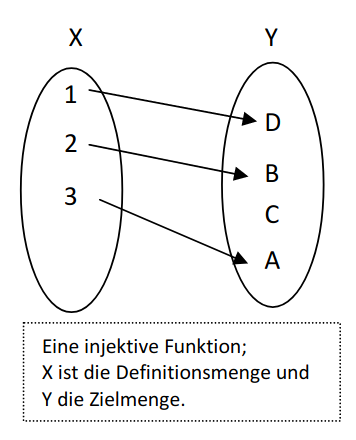
\includegraphics[scale=0.4]{pictures/injektiv}
\end{column}%
\end{columns}
\end{frame}

\begin{frame}{Einschub: Injektiv, Surjektiv, Bijektiv}
\begin{columns}[T] % align columns
\begin{column}{.58\textwidth}
\begin{itemize}
	\item Surjektivität (rechtstotal): Ist eine Eigenschaft einer mathematischen Funktion
	\item Jedes Element der Zielmenge mindestens einmal als Funktionswert angenommen
	\begin{itemize}
		\item Jedes Bild hat mindestens ein Urbild
	\end{itemize}	
	\item Eine surjektive Funktion wird auch als Surjektion bezeichnet
\end{itemize}
\end{column}%
\hfill%
\begin{column}{.38\textwidth}
\centering
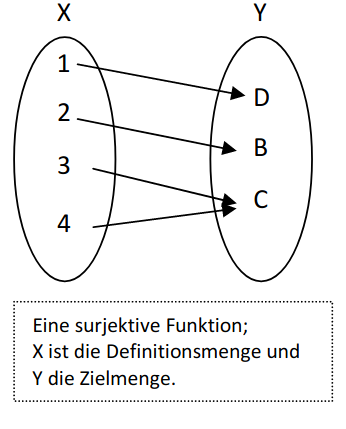
\includegraphics[scale=0.4]{pictures/surjektiv}
\end{column}%
\end{columns}
\end{frame}

\begin{frame}{Einschub: Injektiv, Surjektiv, Bijektiv}
\begin{columns}[T] % align columns
\begin{column}{.58\textwidth}
\begin{itemize}
	\item Bijektivität (bijektiv oder umkehrbar eindeutig auf oder eineindeutig auf) ist eine Eigenschaft einer mathematischen Funktion
	\item Verschiedene Elemente ihres Definitionsbereichs auf verschiedene Elemente der Zielmenge abbildet (injektiv) \textbf{und}
	\item Zusätzlich jedes Element der Zielmenge als Funktionswert auftritt (surjektiv)
	\item Eine bijektive Funktion hat daher immer eine Umkehrfunktion, ist also invertierbar
\end{itemize}
\end{column}%
\hfill%
\begin{column}{.38\textwidth}
\centering
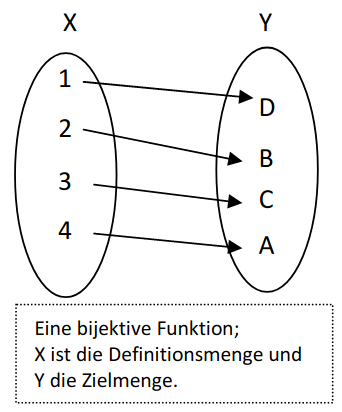
\includegraphics[scale=0.4]{pictures/bijektiv}
\end{column}%
\end{columns}
\end{frame}

\begin{frame}{Rechnen mit natürlichen Zahlen}
\begin{definition}[Addition]
\begin{itemize}
	\item[(A1)] $n + 0 = n$
	\item[(A2)] $n + S(m) = S(n + m)$
\end{itemize}
\end{definition}
Somit ist durch $(S3)$ die Addition $n + m$ für alle $n, m \in \mathbb{N}$ definiert
\begin{block}{Nachweis der Rechenregeln}
\begin{itemize}
	\item Assoziativität: $k + (n + m) = (k + n) + m$
	\item Kommutativität: $n + m = m + n$
\end{itemize}
\end{block}
\textcolor{blue}{Folgerung:} Wir können mit natürlichen Zahlen rechnen\\
\textcolor{red}{Aber:} Bevor wir die Summen zweier konkreter natürlicher Zahlen ausrechnen können, muss jede natürliche Zahl genau einen Namen haben!
\end{frame}

\subsection{Ziffernketten}

\begin{frame}{Ziffernketten}
\textcolor{red}{Problem:} Unendlich viele natürliche Zahlen erfordern unendlich viele Namen.
\textcolor{blue}{Lösung}
\begin{itemize}
	\item Verwende Ziffernketten: $z_1z_2z_3 \ldots z_k \qquad z_i \in \mathcal{Z}, i = 1, \ldots , k$
	\item Endliche Ziffernmenge $\mathcal{Z}$
\end{itemize}

\textcolor{blue}{Interpretation}
\begin{itemize}
	\item Systematische Konstruktion unterschiedlicher Symbole
	\item Bilden von Worten aus einem Alphabet
\end{itemize}
\end{frame}

\subsection{Ziffernsysteme}
\begin{frame}{Ziffernsysteme}
\begin{theorem}
Sei $\mathcal{Z}$ eine endliche Ziffernmenge und
$$
	\mathcal{D} \{z_1z_2 \ldots z_k | k \in \mathbb{N}, z_i \in \mathcal{Z}, i = 1, \ldots, k\}
$$
die Menge aller endlichen Ziffernketten. Dann existiert eine bijektive Abbildung $\varphi : \mathbb{N} \to \mathcal{D}(\mathcal{Z})$
\end{theorem}
\begin{definition}
Die Ziffernmenge $\mathcal{Z}$ und die Zuordnung $\varphi$ erzeugen eine Ziffernsystem zur Darstellung von $\mathbb{N}$
\end{definition}
\begin{definition}
Eine Menge $\mathcal{M}$ , für die eine bijektive Abbildung $\varphi ∶ \mathbb{N} \to \mathcal{M}$ existiert, heißt abzählbar.
\end{definition}
\end{frame}

\begin{frame}{Beispiele für Ziffernsysteme}
\begin{itemize}
	\item Römische Zahlen
	\begin{itemize}
		\item $\mathcal{Z} = \{I, V, X, L, C, D, M\}$
		\item Kein Ziffernsystem!
	\end{itemize}
	\item Unärsystem
	\begin{itemize}
		\item Nur eine Ziffer: $\mathcal{Z} = \{|\}$
		\item Ziffernketten: $\mathcal{D}(\mathcal{Z}) = \{|, ||, |||, \ldots \}$
		\item Zuordnung: $\varphi(0) =, \varphi(1) = |, \varphi(S(n)) = \varphi(n)∣$
		\item Beispiel: $\varphi(4) = ||||$
	\end{itemize}
\end{itemize}
\end{frame}

\begin{frame}{Praktische Anwendung}
\begin{columns}[T] % align columns
\begin{column}{.58\textwidth}
... vor 15000 - 20000 Jahren im Kongo:
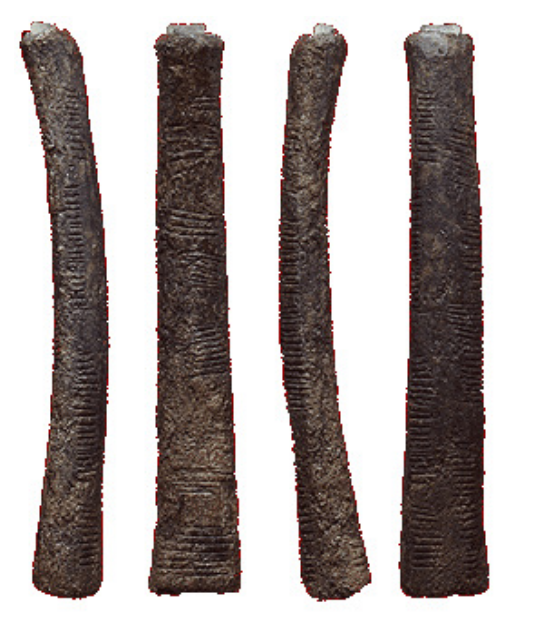
\includegraphics[scale=0.3]{pictures/stick}
\end{column}%
\hfill%
\begin{column}{.38\textwidth}
... heute
\centering
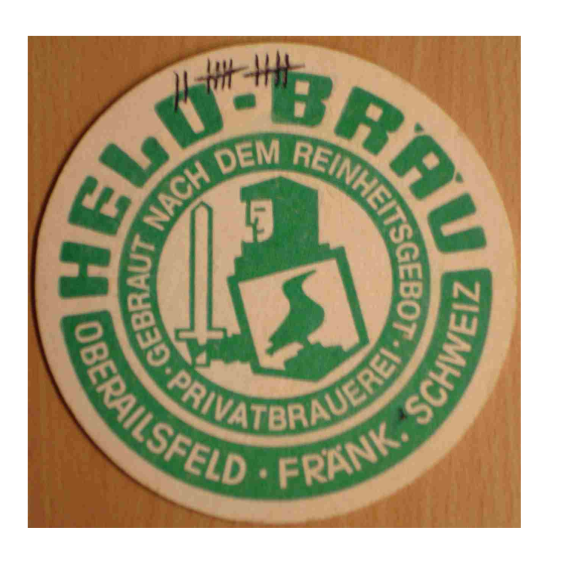
\includegraphics[scale=0.3]{pictures/beer}
\end{column}%
\end{columns}
\end{frame}

\subsection{Potenzzerlegung zur Basis $q$}
\begin{frame}{Potenzzerlegung zur Basis $q$}
\begin{theorem}
Sei $q \in \mathbb{N}, q > 1$ fest gewählt.\\
Dann lässt sich jede Zahl $n \in \mathbb{N}$ als Potenzzerlegung
$$
	n = \sum_{i=0}^k r_i q^i
$$
darstellen.
Die Koeffizienten $r_i \in \{0, \ldots, q-1\} \subset \mathbb{N}$ sind eindeutig.
\end{theorem}
\end{frame}

\subsection{Positionssystem}
\begin{frame}{Positionssystem zur Basis $q$}
\begin{definition}
\begin{itemize}
	\item Ziffernmenge: $\mathcal{Z} = \{z_0 , \ldots , z_{q-1}\}$
	\item Zuordnung:
	$$
		n \mapsto \varphi(n) = z_n, \qquad n = 0, \ldots, q-1
	$$
	und für $n > q-1$
	$$
		n \mapsto \varphi(n) = z_{r_{k}} z_{r_{k-1}} \ldots z_{r_{0}} \qquad \text{ mit } n = \sum_{i=0}^k r_i q^i , \qquad 0 \leq r_i \leq q-1
	$$
\end{itemize}
Diese Zifferndarstellung heißt \textcolor{red}{q-adische} Darstellung.
\end{definition}
\end{frame}

\begin{frame}{Beispiele}
\begin{itemize}
	\item Dezimalsystem
	\begin{itemize}
		\item $q = 10$ und $\mathcal{Z} = \{0, 1, 2, 3, 4, 5, 6, 7, 8, 9\}$
	\end{itemize}
	\item Hexadezimalsystem	
	\begin{itemize}
		\item $q = 16$ und $\mathcal{Z} = \{0, 1, 2, 3, 4, 5, 6, 7, 8, 9, A, B, C, D, E, F \}$
	\end{itemize}
	\item $q$-adische Systeme mit $q \leq 36$
	\begin{itemize}
		\item Erweiterung mit $\{A, B, C, . . . , Z\}$
	\end{itemize}
	\item Konvention:
	\begin{itemize}
		\item Keine Unterscheidung zwischen Darstellung und Zahl:
		$$
			(z_{k}z_{k-1} \ldots z_0)_q = \sum_{i=0}^k z_i q^i , \qquad z_i \in \mathcal{Z} = \{0,1, \ldots q-1 \}
		$$
		\item Kein Index $q$, falls $q = 10$
		\item Den Index $i$ von $z_i$ nennt man Stelle
		\item $(z_{k}z_{k-1} \ldots z_0)$ nennt man eine $k$-stellige Zahl
	\end{itemize}
\end{itemize}
\end{frame}

\subsection{Dualzahlen \& Dualsystem}
\begin{frame}{Positionssystem zur Basis $q = 2$: Dualsystem}
\begin{itemize}
	\item Dualsystem (auch Binärsystem)
	\begin{itemize}
		\item Ziffernmenge: $\mathcal{Z} = \{0, 1\}$
	\end{itemize}
	\item \textcolor{red}{Ideal für technische Umsetzung}
	\begin{itemize}
		\item 1 Binärstelle $\Leftrightarrow$ 1 Bit $\Leftrightarrow$ 1 \enquote{Schalter}
		\item Alle modernen Rechenmaschinen arbeiten mit dem Dualsystem
	\end{itemize}
	\item Zahlenbereich
	\begin{itemize}
		\item Im Dualsystem lassen sich mit $N$ Stellen Zahlen $n \in \mathbb{N}$ mit:
		$$
			0 \leq n \leq 2^{N} - 1
		$$
		darstellen.
	\end{itemize}
\end{itemize}
\end{frame}

\subsection{Technische Realisierung}
\begin{frame}{Technische Realisierung}
\begin{itemize}
	\item Kleinste Einheit (0 oder 1): Bit
	\item Bits werden in festen Längen zusammengefaßt
	\item 8 Bits = 1 Byte mit $2^8 = 256$ verschiedenen Zuständen
	\item Feste Anzahl Bytes für Zahlendarstellung
	\item Bezeichnungen: BYTE, WORD, DWORD, ... (Architekturabhängig)
	\begin{itemize}
		\item Üblich: x\_86/IA32 WORD = 2 Bytes, DWORD = 4 Bytes, QWORD = 8 Bytes
		\item Machineword: Datentyp den die CPU Architektur verarbeiten kann
	\end{itemize}
	\item Bereich von 64-Bit Zahlen
	$$
		0 \leq n \leq 2^{64} - 1 > 18 \cdot 10^{18} = 18 \text{ Trillionen}
	$$
\end{itemize}
\end{frame}

\begin{frame}{Kochrezept Umrechnung ganzer Zahlen}
\begin{center}
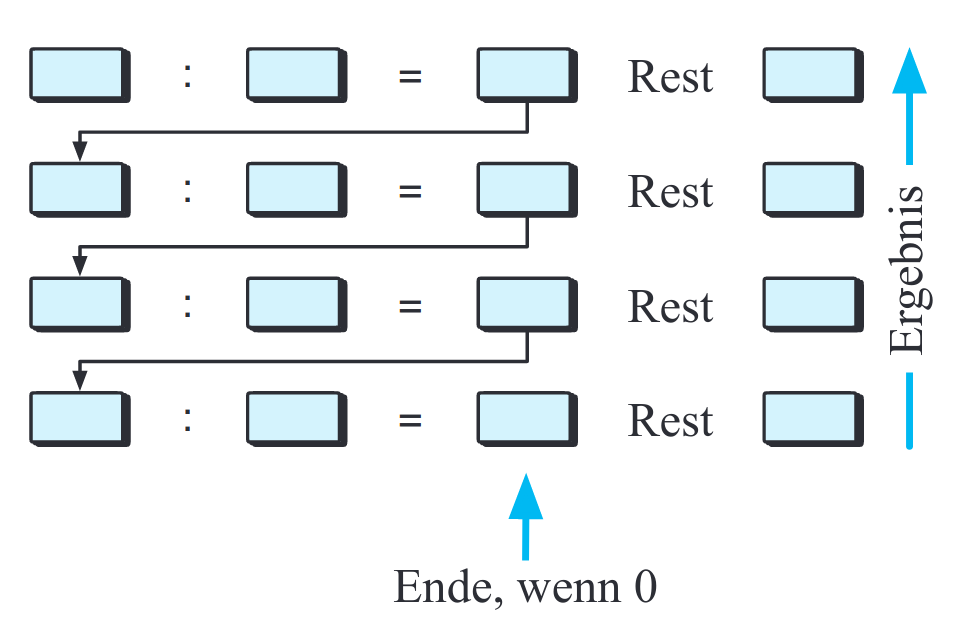
\includegraphics[scale=0.35]{pictures/konv_n}
\end{center}
\end{frame}

\begin{frame}{Beispiel Dualzahlen}
\begin{itemize}
	\item Umrechnung von $741_{10}$ in dual
\end{itemize}
\end{frame}

\section{Umwandlung IN $q$-adische Zahlensysteme}
\subsection{Euklidische Algorithmus}
\begin{frame}{Euklidische Algorithmus}
Umwandlung vom Dezimalsystem in ein Zahlensystem zur Basis $q$
\begin{enumerate}
	\item \textcolor{red}{Methode: Euklidischer Algorithmus:}
	\begin{align*}
		Z &= z_n 10^n + z_{n-1} 10^{n-1} + \ldots + z_1 10^1 + z_0 10^0 + z_{-1} 10^{-1} + \ldots + z_{-m} 10^{-m} \\
		&= y_s q^s + y_{s-1} q^{s-1} + \ldots + y_1 q^1 + y_0 q^0 + y_{-1} q^{-1} + \ldots + y_{-t} q^{-t}
	\end{align*}
\end{enumerate}
Die Ziffern werden sukzessive, beginnend mit der höchstwertigen Ziffer, berechnet:
\begin{enumerate}
	\item \textcolor{red}{Schritt:} Berechne $p$ gemäß der Ungleichung $qp \leq Z < q^{p+1}$\\
	setze $i = p$ und $Z_i = Z$
	\item \textcolor{red}{Schritt:} Ermittle $y_i$ und den Rest $R_i$ durch Division von $Z_i$ durch $q_i$\\
	\textbf{$y_i = Z_i \div q^i$}\\
	\textbf{$R_i = Z_i \mod q^i$}
	\item \textcolor{red}{Schritt:} Wiederhole 2. Schritt für $i = p-1,\ldots$ und ersetze dabei nach jedem Schritt $Z_i$ durch $R_i$, bis $R_i = 0$ oder bis $q^i$ gering genug ist (und damit auch der Umrechnungsfehler).
\end{enumerate}
\end{frame}

\begin{frame}{Beispiel}
Umwandlung von $15741,233_{10}$ ins Hexadezimalsystem
\begin{enumerate}
	\item Schritt $16^3 \leq 15741,233 < 16^4 \Rightarrow$ höchste Potenz $16^3$
\begin{table}[h]
\begin{tabular}{|c|c|c|c|c|c|c|c|}
\cline{1-8}
2.Schritt: & 15741,233 & : & $16^3$ & = & 3 & Rest & $3453,233$ \\ \cline{1-8}
3.Schritt: & 3453,233 & : & $16^2$ & = & D & Rest & $125,233$  \\ \cline{1-8}
4.Schritt & 125,233 & : & $16^1$ & = & 7 & Rest & $13,233$ \\ \cline{1-8}
5.Schritt: & 13,233 & : & $16^0=1$ & = &  D &  Rest & $0,233$ \\ \cline{1-8}
6.Schritt: & 0,233 & : & $16^{-1}$ & = &  3 &  Rest  & $0,0455$ \\ \cline{1-8}
7.Schritt: & 0,0455 & : & $16^{-2}$ & = &  B & Rest & $0,00253$ \\ \cline{1-8}
8.Schritt: & 0,00253 & : & $16^{-3}$ & = & A &  Rest & $0,000088593$ \\ \cline{1-8}
9. Schritt: & 0,000088593 & : & $16^{-4}$ & = & 5 & Rest &  $0,000012299$ \\ \cline{1-8}
\end{tabular}
\end{table}
\begin{center}
	\Rightarrow $15741,233_{10} \approx 3D7D,3BA5_{16}$
\end{center}
\end{enumerate}
\end{frame}

\subsection{Horner Schema}
\begin{frame}{Horner Schema}
Umwandlung vom Dezimalsystem in ein Zahlensystem zur Basis $q$
\begin{enumerate}\addtocounter{enumi}{1}
	\item \textcolor{red}{Methode:} Abwandlung des Horner-Schemas
	\begin{enumerate}
		\item Hierbei müssen der ganzzahlige und der gebrochene Anteil getrennt betrachtet werden.
		\item Umwandlung des ganzzahligen Anteils:
		$$
			\text{Eine ganze Zahl } X_q = \sum_{i=0}^n z_i q^i \text{ kann durch fortgesetztes}
		$$
		Ausklammern auch in folgender Form geschrieben werden:
		$$
			X_q = ((\ldots (((z_n q + z_{n-1}) q + z_{n-2}) q + z_{n-3}) q \ldots ) q + z_1) q + z_0
		$$
	\end{enumerate}
\end{enumerate}
\end{frame}

\begin{frame}{Beispiel}
Die gegebene Dezimalzahl wird sukzessive durch die Basis $q$ \textbf{dividiert}.\\
Die jeweiligen ganzzahligen Reste ergeben die Ziffern der Zahl $X_q$ in der Reihenfolge von der niedrigstwertigen zur höchstwertigen Stelle.\\
Wandle $15741_{10}$ ins Hexadezimalsystem
\end{frame}

\begin{frame}{Beispiel}
Die gegebene Dezimalzahl wird sukzessive durch die Basis $q$ \textbf{dividiert}.\\
Die jeweiligen ganzzahligen Reste ergeben die Ziffern der Zahl $X_q$ in der Reihenfolge von der niedrigstwertigen zur höchstwertigen Stelle.\\
Wandle $15741_{10}$ ins Hexadezimalsystem
\begin{table}[h]
\begin{tabular}{cccccc}
1574110 : 16 & = & 983 & Rest & 13 & $D_{16}$ \\ 
98310 : 16 & = & 61 & Rest & 7 & ($7_{16}$) \\
6110 : 16 & = &  3 & Rest & 13 & ($D_{16}$) \\
310 : 16 & = & 0 & Rest & 3 & ($3_{16}$)
\end{tabular}
\end{table}
\begin{center}
	$$ \Rightarrow 15741_{10} = 3D7D_{16}$$
\end{center}
\end{frame}

\begin{frame}{Umwandlung des Nachkommateils}
Auch der gebrochene Anteil einer Zahl $$Y_q = \sum_{i=-m}^{-1} y_i q^i$$ lässt sich entsprechend schreiben:
$$
	Y_q = ((\ldots ((y_{-m} q^{-1} + y_{-m+1}) q^{-1} + y_{-m+2}) b^{-1} + \ldots +y_{-2}) q^{-1} + y_{-1}) b^{-1}
$$
\textbf{Verfahren:}\\
Eine sukzessive \textbf{Multiplikation} des Nachkommateils der Dezimalzahl mit der Basis $q$ des Zielsystems ergibt nacheinander die $y_{-i}$ in der Reihenfolge der höchstwertigen zur niedrigstwertigen Nachkommaziffer.
\end{frame}

\begin{frame}{Beispiel}
Umwandlung von $0,233_{10}$ ins Hexadezimalsystem:
\begin{figure}
\center
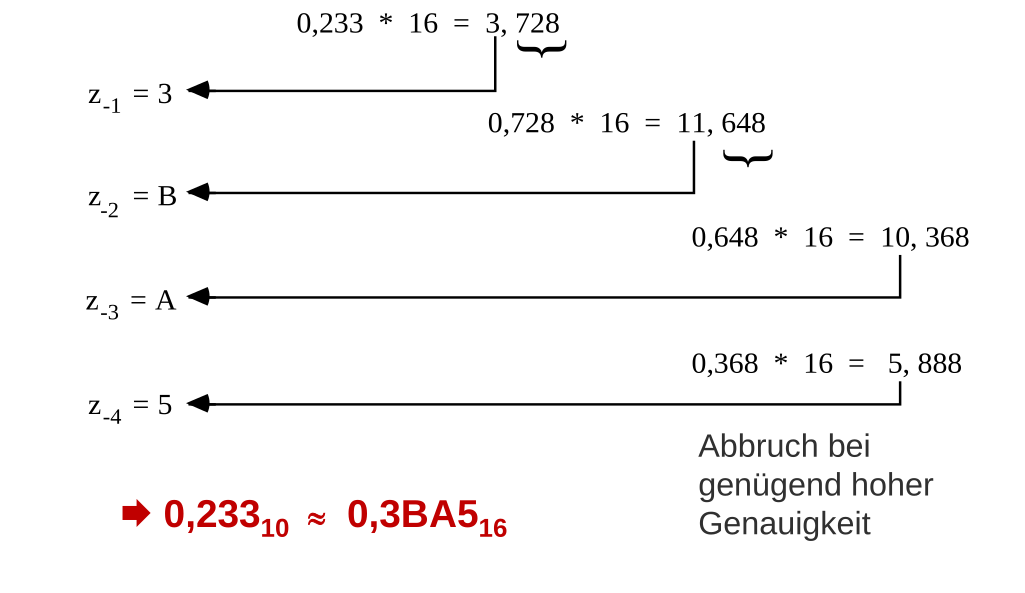
\includegraphics[scale=0.3]{pictures/horner2.png}
\end{figure}
\end{frame}

\section{Umwandlung ins Dezimalsystem}

\begin{frame}{Umwandlung: Basis $q \to$ Dezimalsystem}
Die Werte der einzelnen Stellen der umzuwandelnden Zahl werden in dem Zahlensystem, in das umgewandelt werden soll, dargestellt und nach der Stellenwertgleichung aufsummiert.\\
Der Wert $X_q$ der Zahl ergibt sich dann als Summe der Werte aller Einzelstellen $z_i q^i$:
\begin{align*}
	X_q &= z_n q^n + z_{n -1} q^{n - 1} + \ldots + z_1 q^1 + z_0 q^0 + z_{-1} q^{-1} + \ldots + z_{-m} q^{-m}\\ 		&= \sum_{i=-m}^n z_i q^i
\end{align*}
\end{frame}

\begin{frame}{Beispiel}
Konvertierung $101101,1101_2$ ins Dezimalsystem
\begin{figure}
\hspace{-1.7cm}
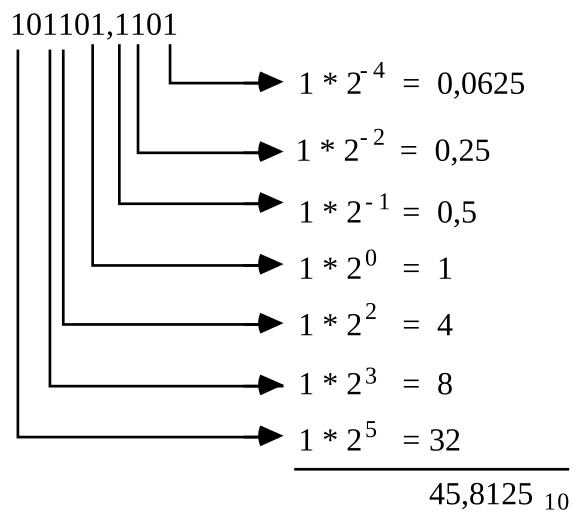
\includegraphics[scale=0.37]{pictures/bin_dec}
\end{figure}
\end{frame}

\subsection{Verallgemeinerung}
\begin{frame}{Umwandlung beliebiger Stellenwertsysteme}
Man wandelt die Zahl ins Dezimalsystem um und führt danach mit Methode 1 oder 2 die Wandlung ins Zielsystem
durch.\\
Spezialfall:
\begin{itemize}
	\item Ist eine Basis eine Potenz der anderen Basis, können einfach mehrere Stellen zu einer Ziffer zusammengefasst werden oder eine Stelle kann durch eine Folge von Ziffern ersetzt werden.
\end{itemize}
Wandlung von $0110100,110101_2$ ins Hexadezimalsystem als BYTE dargestellt
$2^4 = 16 \Rightarrow 4$ Dualstellen $\to$ 1 Hexadezimalstellen
\begin{align*}
\text{dual}\qquad & 0110100,110101 \\
	& \qquad \qquad \downarrow \\
 & \underbrace{0011} \underbrace{0100} , \underbrace{1101} \underbrace{0100}\\
\text{hex}\qquad & \quad 3 \quad~ 4 ~~~, ~ D \quad ~~4
\end{align*}
Ergänzen von Nullen zum Auffüllen auf Vierergruppen
\end{frame}

\section*{Quellen}
\appendix
\begin{frame}[allowframebreaks]
  \frametitle<presentation>{Quellen}
\printbibliography
\end{frame}
\end{document}